\begin{frame}{}
    \centering
    \LARGE Autoregressive Models: \textbf{Modern Models}
\end{frame}

\begin{frame}[allowframebreaks]{Autoregressive Models: Modern Models}
    Modern autoregressive models are powerful tools for generating data like images, audio, and text. Let’s look at some popular ones and why they matter:

    \begin{itemize}
        \item \textbf{PixelCNN/PixelSNAIL:} Great for generating images, using special convolutions to look at pixels one by one.
        \item \textbf{WaveNet:} Designed for audio, it can create realistic speech and music by looking at sound samples in order.
        \item \textbf{Transformer-based Models:} Used in language models like GPT, these use attention to understand and generate sequences (text, images, etc.).
    \end{itemize}

    \framebreak

    \textbf{PixelCNN/PixelSNAIL:}
    \begin{itemize}
        \item PixelCNN was introduced in 2016 to generate images pixel by pixel.
        \item It uses masked convolutions so each pixel only depends on the ones before it.
        \item PixelSNAIL improves on this by adding attention, helping the model see more of the image at once.
        \item Both are good at making realistic images.
    \end{itemize}

    \framebreak

    \textbf{WaveNet:}
    \begin{itemize}
        \item WaveNet was made for audio generation, like speech and music.
        \item It uses dilated convolutions to look at long stretches of audio.
        \item Each sound sample depends on the previous ones, making the output sound natural.
        \item WaveNet set new standards for speech synthesis.
    \end{itemize}

    \framebreak

    \textbf{Transformer-based Models:}
    \begin{itemize}
        \item Transformers were introduced in 2017 for language tasks.
        \item They use self-attention to look at all parts of a sequence at once.
        \item This makes them fast and good at handling long texts or sequences.
        \item Famous models like GPT-3 and BERT use this idea.
        \item Transformers can also be used for images and audio, not just text.
    \end{itemize}

    \framebreak

    \textbf{Applications:}
    \begin{itemize}
        \item Making new images (PixelCNN, PixelSNAIL)
        \item Generating speech and music (WaveNet)
        \item Writing text and language modeling (Transformers)
        \item Creating videos and working with multiple types of data
    \end{itemize}

    \framebreak

    \textbf{Pros:}
    \begin{itemize}
        \item Can generate high-quality images, audio, and text
        \item Good at learning complex patterns in data
        \item Scalable to large datasets and tasks
    \end{itemize}

    \textbf{Cons:}
    \begin{itemize}
        \item Training and running these models can be expensive
        \item Need lots of data to work well
        \item Still challenging for very large or complex data
    \end{itemize}
\end{frame}
\begin{frame}[allowframebreaks]{PixelCNN}
\textbf{Masked Spatial (2D) Convolution - PixelCNN}
\begin{itemize}
    \item Images can be flattened into 1D vectors, but they are fundamentally 2D.
    \item We can use a masked variant of ConvNet to exploit this knowledge.
    \item First, we impose an autoregressive ordering on 2D images:
\end{itemize}

\begin{figure}
    \centering
    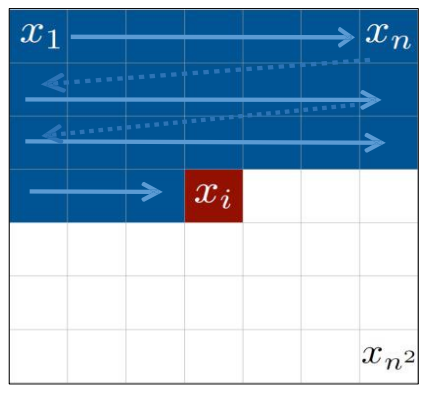
\includegraphics[height=0.4\textheight, width=\textwidth,keepaspectratio]{images/autoregressive/raster-scan.png}
    \caption*{Raster scan ordering of a 2D image. The pixels are processed in a left-to-right, top-to-bottom manner, similar to reading text.}
\end{figure}

\framebreak
\begin{itemize}
    \item The autoregressive ordering allows us to use a convolutional neural network (CNN) to predict the next pixel based on the previously generated pixels.
    \item We use masked convolutions to ensure that the model only has access to the pixels that have already been generated.
    \item The convolutional layers are designed to respect the autoregressive ordering, meaning that each pixel is predicted based on its left and top neighbours, but not the right or bottom neighbours.
\end{itemize}
\framebreak
\textbf{PixelCNNs}: Use the neighbour pixels to predict the new pixel.
\begin{columns}
        \begin{column}{0.5\textwidth}
            \begin{figure}
                \centering
                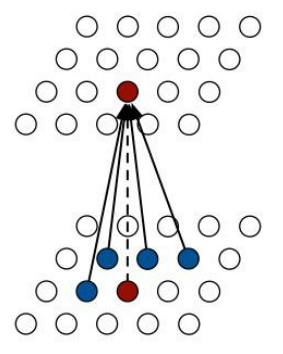
\includegraphics[width=0.9\textwidth, keepaspectratio]{images/autoregressive/pixelcnn.png}
                \caption*{Image generation with pixelCNN}
            \end{figure}
        \end{column}
        \begin{column}{0.5\textwidth}
            \begin{figure}
                \centering
                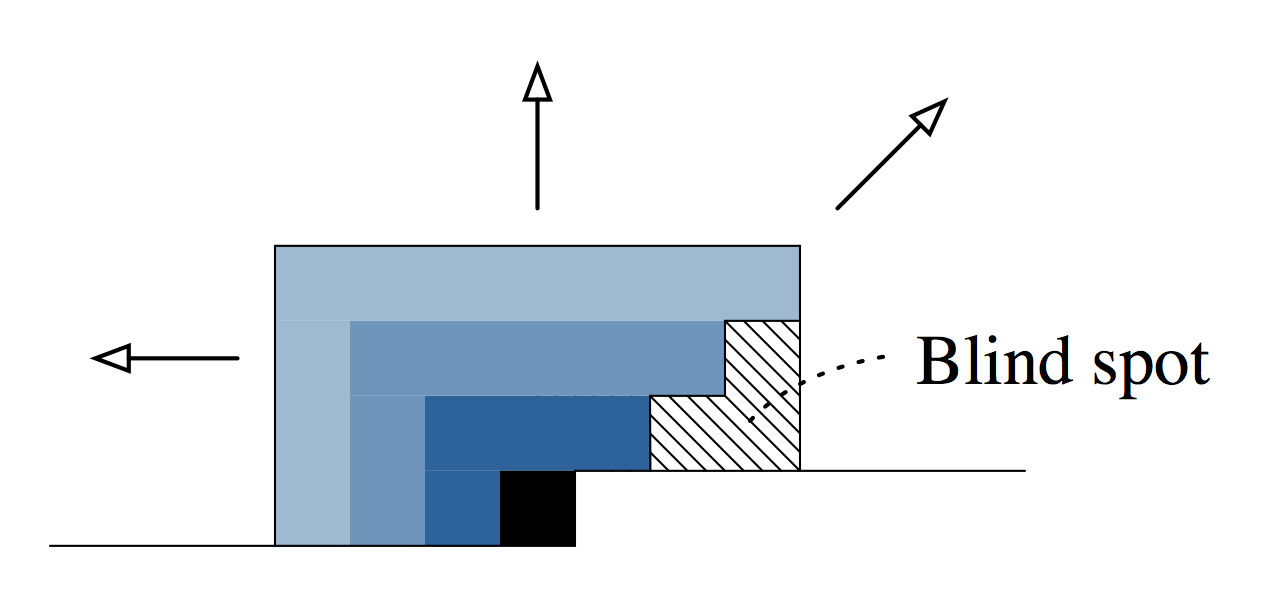
\includegraphics[width=1.1\textwidth,keepaspectratio]{images/autoregressive/pixelcnn-blindspot.png}
                \caption*{PixelCNN-style masking has one problem: blind spot in receptive field. The model cannot see the pixels to the right and below the current pixel, which can lead to artifacts in generated images.}
            \end{figure}
        \end{column}
    \end{columns}

\framebreak

\begin{itemize}
    \item PixelCNN results
        \begin{figure}
        \centering
        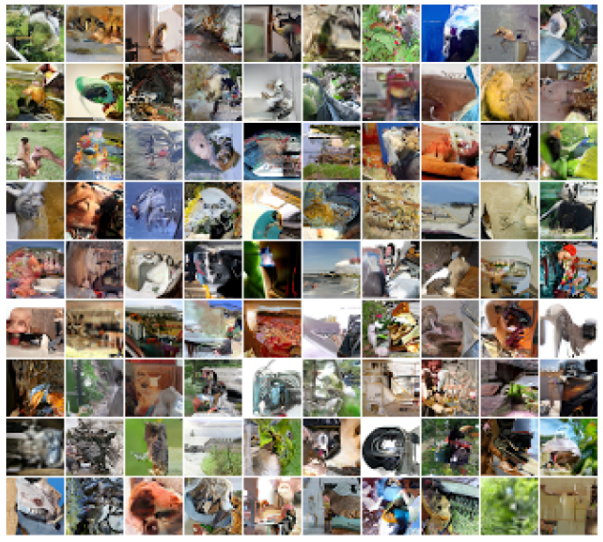
\includegraphics[height=0.65\textheight, width=\textwidth, keepaspectratio]{images/autoregressive/pixelcnn_results.png}
        \caption*{Image generation with pixelCNN. Model trained on Imagenet (32 x 32 pixels)}
    \end{figure}
\end{itemize}
\end{frame}
\begin{frame}[allowframebreaks]{WaveNet}
    % --- Causal Convolution ---
    \begin{columns}
        \begin{column}{0.6\linewidth}
            \begin{figure}
                \centering
                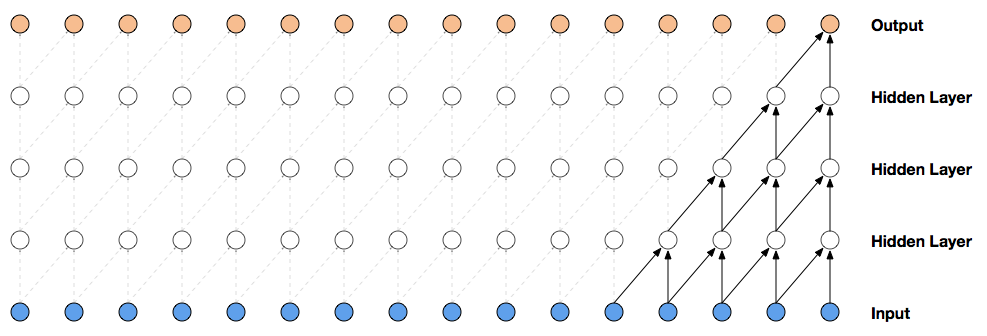
\includegraphics[width=1\linewidth]{images/autoregressive/casual-convolution.png}
                \caption*{Visualization of a stack of causal convolutional layers.}
            \end{figure}
        \end{column}
        \begin{column}{0.5\linewidth}
            \begin{itemize}
                \item \textbf{Causal convolution:} Each output depends only on current and previous inputs.
                \item Easy to implement: masking part of the convolution kernel.
                \item Constant parameter count for variable-length distributions.
                \item Efficient to compute: convolution has hyper-optimized implementations on all hardware.
                \item[] \textbf{However:}
                \begin{itemize}
                    \item Limited receptive field, grows linearly with the number of layers.
                \end{itemize}
            \end{itemize}
        \end{column}
    \end{columns}
    \small [WaveNet – Van den Oord et al, 2016]

    \framebreak

    % --- Softmax Output Distribution ---
    \textbf{Softmax Output Distribution}

    \begin{itemize}
        \item WaveNet models the conditional distribution of the next sample as a categorical distribution:
    \end{itemize}
    \begin{equation*}
        p(x_t | x_{1}, \ldots, x_{t-1}) = \mathrm{Softmax}(f(x_{1}, \ldots, x_{t-1}))
    \end{equation*}
    \begin{itemize}
        \item The output at each timestep is a probability distribution over possible quantized values.
        \item Typically, 8-bit $\mu$-law quantization is used for audio.
    \end{itemize}

    \framebreak

    % --- Dilated Convolutions ---
    \begin{columns}
        \begin{column}{0.6\linewidth}
            \begin{figure}
                \centering
                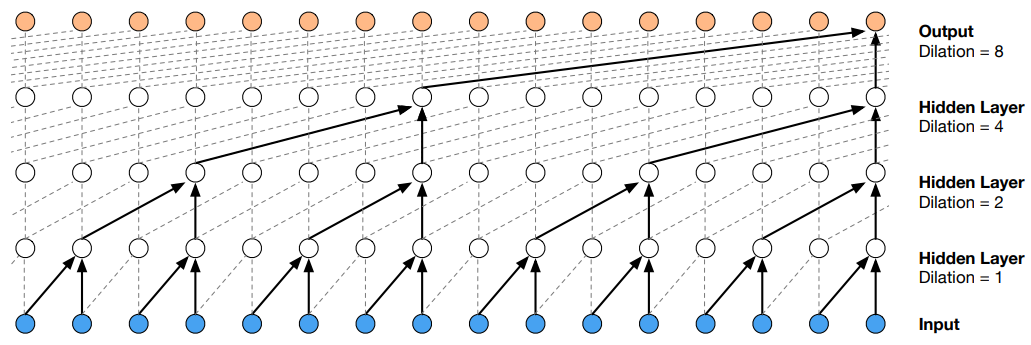
\includegraphics[width=1\linewidth]{images/autoregressive/dilated-casual-convolution.png}
                \caption*{Visualization of a stack of \textit{dilated} causal convolutional layers.}
            \end{figure}
        \end{column}
        \begin{column}{0.5\linewidth}
            \begin{itemize}
                \item \textbf{Dilated convolution:} Expands receptive field exponentially with depth.
                \item Dilation factor $d$:
                \begin{equation*}
                    y[t] = \sum_{k=0}^{K-1} w[k] \cdot x[t - d \cdot k]
                \end{equation*}
                \item Enables efficient modeling of long-range dependencies.
            \end{itemize}
        \end{column}
    \end{columns}
    \small [WaveNet – Van den Oord et al, 2016]

    \framebreak

    % --- Gated Activation Units ---
    \textbf{Gated Activation Units}

    \begin{itemize}
        \item Each residual block uses gated activation units:
    \end{itemize}
    \begin{equation*}
        z = \tanh(W_{f} * x) \odot \sigma(W_{g} * x)
    \end{equation*}
    \begin{itemize}
        \item $W_{f}$, $W_{g}$: convolution filters for filter and gate.
        \item $\odot$: element-wise multiplication.
        \item $\sigma$: sigmoid activation.
        \item Improves expressivity and helps gradient flow.
    \end{itemize}

    \framebreak

    % --- Residual and Skip Connections ---
    \textbf{Residual and Skip Connections}

    \begin{columns}
        \begin{column}{0.6\linewidth}
            \begin{figure}
                \centering
                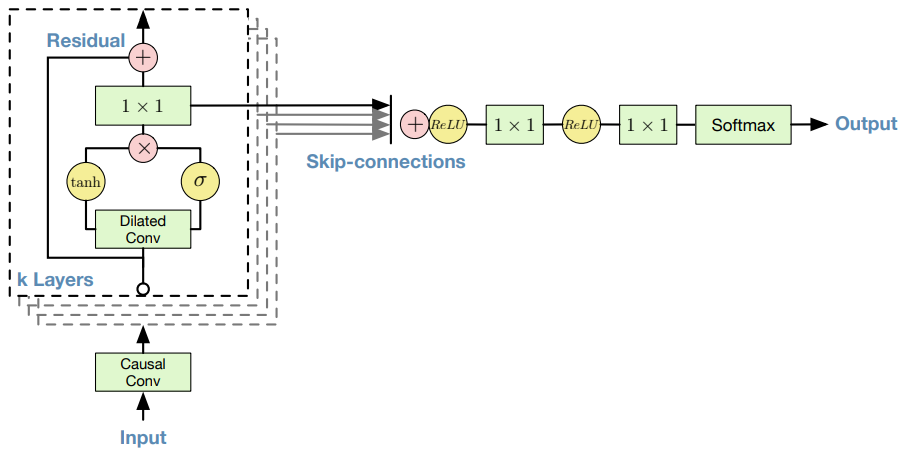
\includegraphics[width=1\linewidth]{images/autoregressive/architecture-residual-block.png}
                \caption*{Overview of the residual block and the entire architecture.}
            \end{figure}
        \end{column}
        \begin{column}{0.5\linewidth}
            \begin{itemize}
                \item \textbf{Residual connections:} Add input to output of each block.
                \item \textbf{Skip connections:} Aggregate outputs from all blocks before final output.
                \item Helps training deep networks and improves convergence.
            \end{itemize}
        \end{column}
    \end{columns}

    \framebreak

    % --- Conditional WaveNet ---
    \textbf{Conditional WaveNet}

    \begin{itemize}
        \item WaveNet can be conditioned on additional information (e.g., speaker identity, linguistic features).
        \item Conditioning vector $h$ is added to each layer:
    \end{itemize}
    \begin{equation*}
        z = \tanh(W_{f} * x + V_{f} * h) \odot \sigma(W_{g} * x + V_{g} * h)
    \end{equation*}
    \begin{itemize}
        \item Enables applications like text-to-speech (TTS) and voice conversion.
    \end{itemize}

    \framebreak

    % --- Context Stacks ---
    \textbf{Context Stacks}

    \begin{itemize}
        \item Multiple stacks of dilated convolutions with different dilation rates.
        \item Each stack captures dependencies at different temporal scales.
        \item Improves model's ability to capture both short-term and long-term context.
    \end{itemize}
    \begin{equation*}
        \text{Stack}_i: \quad d \in \{1, 2, 4, \ldots, 2^{n-1}\}
    \end{equation*}

    \framebreak

    \textbf{\large WaveNet on MNIST}
    \vspace{2em}
    \begin{columns}
        \begin{column}{0.18\linewidth}
            \begin{figure}
                \centering
                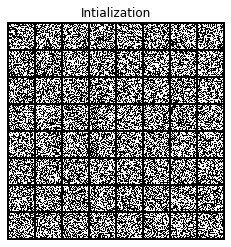
\includegraphics[width=1\linewidth]{images/autoregressive/mnist/init.png}
            \end{figure}
        \end{column}
        \begin{column}{0.18\linewidth}
            \begin{figure}
                \centering
                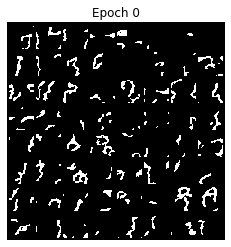
\includegraphics[width=1\linewidth]{images/autoregressive/mnist/epoch-0.png}
            \end{figure}
        \end{column}
        \begin{column}{0.18\linewidth}
            \begin{figure}
                \centering
                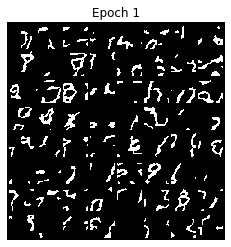
\includegraphics[width=1\linewidth]{images/autoregressive/mnist/epoch-1.png}
            \end{figure}
        \end{column}
        \begin{column}{0.18\linewidth}
            \begin{figure}
                \centering
                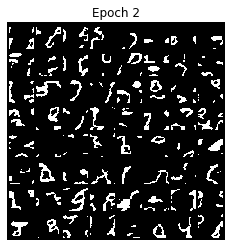
\includegraphics[width=1\linewidth]{images/autoregressive/mnist/epoch-2.png}
            \end{figure}
        \end{column}
        \begin{column}{0.18\linewidth}
            \begin{figure}
                \centering
                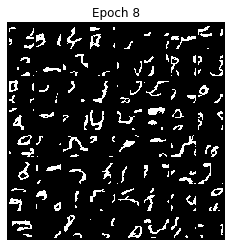
\includegraphics[width=1\linewidth]{images/autoregressive/mnist/epoch-8.png}
            \end{figure}
        \end{column}
        \begin{column}{0.18\linewidth}
            \begin{figure}
                \centering
                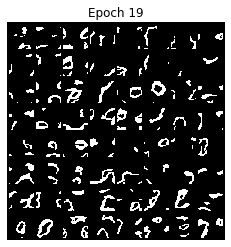
\includegraphics[width=1\linewidth]{images/autoregressive/mnist/epoch-19.png}
            \end{figure}
        \end{column}
    \end{columns}

    \framebreak

    \textbf{\large WaveNet with Pixel Location Appended on MNIST} \\
    \vspace{2em}
    Append (x,y) coordinates of pixel in the image as input to WaveNet
    \vspace{1em}
    \begin{columns}
        \begin{column}{0.18\linewidth}
            \begin{figure}
                \centering
                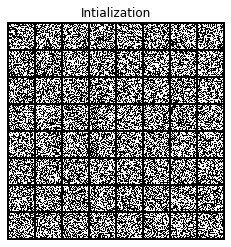
\includegraphics[width=1\linewidth]{images/autoregressive/mnist/init.png}
            \end{figure}
        \end{column}
        \begin{column}{0.18\linewidth}
            \begin{figure}
                \centering
                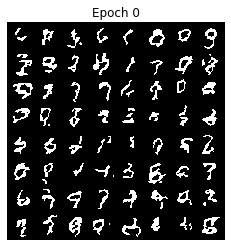
\includegraphics[width=1\linewidth]{images/autoregressive/mnist/coord-epoch-0.png}
            \end{figure}
        \end{column}
        \begin{column}{0.18\linewidth}
            \begin{figure}
                \centering
                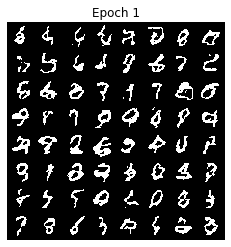
\includegraphics[width=1\linewidth]{images/autoregressive/mnist/coord-epoch-1.png}
            \end{figure}
        \end{column}
        \begin{column}{0.18\linewidth}
            \begin{figure}
                \centering
                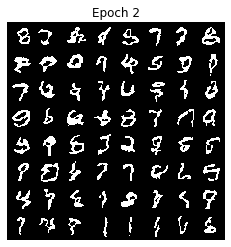
\includegraphics[width=1\linewidth]{images/autoregressive/mnist/coord-epoch-2.png}
            \end{figure}
        \end{column}
        \begin{column}{0.18\linewidth}
            \begin{figure}
                \centering
                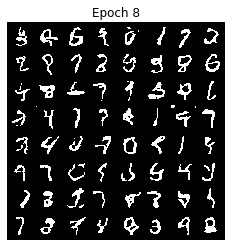
\includegraphics[width=1\linewidth]{images/autoregressive/mnist/coord-epoch-8.png}
            \end{figure}
        \end{column}
        \begin{column}{0.18\linewidth}
            \begin{figure}
                \centering
                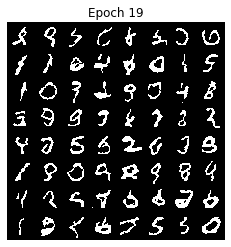
\includegraphics[width=1\linewidth]{images/autoregressive/mnist/coord-epoch-19.png}
            \end{figure}
        \end{column}
    \end{columns}

    \framebreak

    % --- Summary ---
    \textbf{WaveNet} is a deep generative model for raw audio waveforms, introduced by DeepMind in 2016. It models the conditional probability of the next audio sample given all previous samples using stacks of causal, dilated convolutional layers.

    \begin{itemize}
        \item \textbf{Autoregressive}: Predicts each audio sample sequentially, conditioning on previous samples.
        \item \textbf{Dilated Convolutions}: Enables the model to capture long-range temporal dependencies efficiently.
        \item \textbf{Gated Units, Residual/Skip Connections}: Improve expressivity and trainability.
        \item \textbf{Conditional WaveNet}: Allows conditioning on external features.
        \item \textbf{Applications}: High-quality text-to-speech (TTS), music generation, and audio synthesis.
        \item \textbf{Advantages}: Produces highly realistic and natural-sounding audio compared to previous methods.
    \end{itemize}
\end{frame}